%% METADATA
%% subject-code: DI01000061
%% subject-name: Modern Physics
%% semester: 1
%% examination: Winter-2024
%% date: 09-01-2025
%% description: Solution guide for Modern Physics (DI01000061)
%% tags: study-material, solutions, gtu, DI01000061, physics
%% END METADATA

\documentclass{article}

% content/resources/templates/preamble.tex
\usepackage[margin=0.6in]{geometry}
\author{Milav Dabgar}
\usepackage{amsmath,amssymb,amsthm}
\usepackage{booktabs}
\usepackage{multirow}
\usepackage{xcolor}
\usepackage{tcolorbox}
\tcbuselibrary{breakable,skins}
\usepackage[colorlinks=true,linkcolor=blue]{hyperref}
\usepackage{titlesec}
\usepackage{enumitem}
\usepackage{tikz}
\usepackage{pgfplots}
\usepackage{circuitikz}
\usepackage[version=4]{mhchem}
\usepackage{longtable}
\usepackage{array}
\usepackage{float}
\usepackage{caption}
\usepackage{listings}

\lstset{
  basicstyle=\small\ttfamily,
  breaklines=true,
  breakatwhitespace=false,
  postbreak=\mbox{\textcolor{red}{$\hookrightarrow$}\space},
  float=false,
  numbers=left,
  numberstyle=\tiny\color{gray},
  numbersep=10pt,
  xleftmargin=2em,
  keywordstyle=\color{blue},
  commentstyle=\color{green!60!black},
  stringstyle=\color{purple},
  backgroundcolor=\color{gray!5},
  showstringspaces=false,
  tabsize=2,
  captionpos=b,
  keepspaces=true,
  columns=flexible
}

\pgfplotsset{compat=1.18}
\usetikzlibrary{shapes,arrows,positioning,calc,patterns,decorations.pathmorphing,decorations.markings,arrows.meta}

% Color scheme
\definecolor{headcolor}{RGB}{0,102,204}
\definecolor{keycolor}{RGB}{220,20,60}
\definecolor{solutioncolor}{RGB}{34,139,34}
\definecolor{mnemoniccolor}{RGB}{148,0,211}
\definecolor{codecolor}{RGB}{0,0,100}

% Spacing
\setlength{\parskip}{3pt}
\setlist[itemize]{nosep}
\setlist[enumerate]{nosep}

% Title formatting
\titleformat{\section}{\Large\bfseries\color{headcolor}}{\thesection}{1em}{}
\titleformat{\subsection}{\large\bfseries\color{headcolor}}{\thesubsection}{1em}{}

% Pandoc tightlist compatibility
\providecommand{\tightlist}{%
  \setlength{\itemsep}{0pt}\setlength{\parskip}{0pt}}

% Pandoc longtable compatibility
\newcounter{none}
\def\thenone{}


\title{Modern Physics (DI01000061) - Winter 2024 Solution}
\date{January 9, 2025}

\hypersetup{
  pdftitle={Modern Physics (DI01000061) - Winter 2024 Solution},
  pdfsubject={GTU Exam Solution - Winter-2024},
  pdfauthor={Milav Dabgar},
  pdfkeywords={study-material, solutions, gtu, DI01000061, physics},
  pdfcreator={pdflatex}
}

\begin{document}
\maketitle

\setcounter{tocdepth}{5}
\tableofcontents
\newpage

% ========================================
% QUESTION 1: MCQs and Fill in the Blanks (14 marks)
% Demonstrates: Short answer format, multiple topics
% ========================================

\section{Question 1}
\textbf{Fill in the blanks/MCQs using appropriate choice from the given options.}

\subsection{Question 1(1) [1 marks]}
\textbf{Which of the following is a semiconductor?}

\textbf{Options:} (a) Si (b) Cu (c) Fe (d) Ni

\subsubsection{Solution}
\paragraph{Answer:} (a) Si

\paragraph{Explanation:}
Silicon (Si) is a Group 14 element with 4 valence electrons, making it an intrinsic semiconductor. Copper (Cu), Iron (Fe), and Nickel (Ni) are metals with high electrical conductivity due to free electrons.

\subparagraph{Note:} Germanium (Ge) is also a semiconductor from Group 14.

\paragraph{Mnemonic:} \emph{Si = Semiconductor, Cu/Fe/Ni = Metals.}

\subsection{Question 1(2) [1 marks]}
\textbf{Refractive index of glass is \_\_\_\_\_.}

\textbf{Options:} (a) 1.50 (b) 1.33 (c) 1.00 (d) 2.43

\subsubsection{Solution}
\paragraph{Answer:} (a) 1.50

\paragraph{Explanation:}
The refractive index of ordinary glass is approximately 1.50. Water has \(n = 1.33\), air/vacuum has \(n = 1.00\), and diamond has \(n = 2.43\).

\subparagraph{Note:} Higher refractive index means light travels slower in that medium.

\paragraph{Mnemonic:} \emph{Glass = 1.5, Water = 1.33, Diamond = 2.43.}

\subsection{Question 1(3) [1 marks]}
\textbf{When an angle of incidence becomes \_\_\_\_\_ critical angle, total internal reflection occurs.}

\textbf{Options:} (a) equal to (b) greater than (c) less than (d) none of these

\subsubsection{Solution}
\paragraph{Answer:} (b) greater than

\paragraph{Explanation:}
Total Internal Reflection (TIR) occurs when light travels from denser to rarer medium and the angle of incidence \(i\) is greater than the critical angle \(C\), i.e., \(i > C\).

\paragraph{Mnemonic:} \emph{TIR when i > C (Greater than Critical).}

\subsection{Question 1(4) [1 marks]}
\textbf{How many P-N junction diodes are used in a Bridge rectifier?}

\textbf{Options:} (a) 2 (b) 3 (c) 4 (d) 5

\subsubsection{Solution}
\paragraph{Answer:} (c) 4

\paragraph{Explanation:}
A bridge rectifier uses 4 diodes arranged in a bridge configuration to convert AC to full-wave DC. This allows current flow through the load in the same direction during both half cycles.

\paragraph{Mnemonic:} \emph{Bridge = 4 Diodes.}

\subsection{Question 1(5) [1 marks]}
\textbf{Optical fiber works on the principle of \_\_\_\_\_.}

\textbf{Options:} (a) Interference (b) Refraction (c) Polarization (d) Total internal reflection

\subsubsection{Solution}
\paragraph{Answer:} (d) Total internal reflection

\paragraph{Explanation:}
Optical fibers transmit light signals by repeated total internal reflection at the core-cladding interface, where the core has a higher refractive index than the cladding.

\paragraph{Mnemonic:} \emph{Fiber = TIR (Total Internal Reflection).}

\subsection{Question 1(6) [1 marks]}
\textbf{Number of oscillations performed per unit time is called \_\_\_\_\_.}

\textbf{Options:} (a) periodic time (b) wavelength (c) amplitude (d) frequency

\subsubsection{Solution}
\paragraph{Answer:} (d) frequency

\paragraph{Explanation:}
Frequency (\(f\)) is defined as the number of complete oscillations per unit time. Its unit is Hertz (Hz) or \(s^{-1}\). The relationship is \(f = 1/T\), where \(T\) is the periodic time.

\paragraph{Mnemonic:} \emph{Frequency = Oscillations per second.}

\subsection{Question 1(7) [1 marks]}
\textbf{The S.I. unit of electric charge is \_\_\_\_\_.}

\textbf{Options:} (a) Coulomb (b) Ampere (c) Volt (d) Faraday

\subsubsection{Solution}
\paragraph{Answer:} (a) Coulomb

\paragraph{Explanation:}
The SI unit of electric charge is Coulomb (C). One Coulomb is the charge transported by a current of one Ampere in one second (\(1\,C = 1\,A \times 1\,s\)).

\paragraph{Mnemonic:} \emph{Charge = Coulomb (C).}

\subsection{Question 1(8) [1 marks]}
\textbf{If the periodic time of simple pendulum is 2 second, then its frequency will be \_\_\_\_\_.}

\textbf{Options:} (a) 2 Hz (b) 0.5 Hz (c) 0.2 Hz (d) 5 Hz

\subsubsection{Solution}
\paragraph{Answer:} (b) 0.5 Hz

\paragraph{Explanation:}
The relationship between frequency (\(f\)) and periodic time (\(T\)) is inverse. Frequency tells us how many complete cycles occur per second, while period tells us how long one cycle takes.

\paragraph{Calculation:}
\[ f = \frac{1}{T} = \frac{1}{2} = 0.5 \, \text{Hz} \]

\paragraph{Mnemonic:} \emph{f = 1/T.}

\subsection{Question 1(9) [1 marks]}
\textbf{The velocity of light is \_\_\_\_\_ in vacuum.}

\textbf{Options:} (a) 300000 km/s (b) 300000 m/s (c) 341 km/s (d) 341 m/s

\subsubsection{Solution}
\paragraph{Answer:} (a) 300000 km/s

\paragraph{Explanation:}
The speed of light in vacuum is \(c = 3 \times 10^8\,m/s = 300000\,km/s\). This is a fundamental constant in physics. Note: 341 m/s is the speed of sound in air.

\paragraph{Mnemonic:} \emph{c = 3\texttimes10\textsuperscript{8} m/s = 300000 km/s.}

\subsection{Question 1(10) [1 marks]}
\textbf{The velocity of sound waves is maximum in \_\_\_\_\_.}

\textbf{Options:} (a) liquid (b) solid (c) gas (d) vacuum

\subsubsection{Solution}
\paragraph{Answer:} (b) solid

\paragraph{Explanation:}
Sound travels fastest in solids due to closely packed molecules and strong intermolecular forces. Order: \(v_{solid} > v_{liquid} > v_{gas}\). Sound cannot travel in vacuum.

\paragraph{Mnemonic:} \emph{Solids = Fastest sound.}

\subsection{Question 1(11) [1 marks]}
\textbf{The propagation of light wave is due to \_\_\_\_\_.}

\textbf{Options:} (a) crest and trough (b) compression and rarefaction (c) only compression (d) only rarefaction

\subsubsection{Solution}
\paragraph{Answer:} (a) crest and trough

\paragraph{Explanation:}
Light waves are transverse electromagnetic waves that propagate through alternating crests and troughs. Compression and rarefaction are associated with longitudinal waves like sound.

\paragraph{Mnemonic:} \emph{Light = Transverse = Crest/Trough.}

\subsection{Question 1(12) [1 marks]}
\textbf{LASER radiation is \_\_\_\_\_.}

\textbf{Options:} (a) polychromatic (b) monochromatic (c) low intense (d) none of these

\subsubsection{Solution}
\paragraph{Answer:} (b) monochromatic

\paragraph{Explanation:}
LASER (Light Amplification by Stimulated Emission of Radiation) produces monochromatic light, meaning it has a single precise wavelength. It is also coherent and highly intense.

\paragraph{Mnemonic:} \emph{LASER = Monochromatic, Coherent, Directional.}

\subsection{Question 1(13) [1 marks]}
\textbf{Which fiber provides longer bandwidth?}

\textbf{Options:} (a) Single mode (b) Multi mode step index (c) Step index (d) None of these

\subsubsection{Solution}
\paragraph{Answer:} (a) Single mode

\paragraph{Explanation:}
Single mode fibers have a very small core diameter and allow only one mode of light propagation, resulting in minimal dispersion and maximum bandwidth. They are used for long-distance communication.

\paragraph{Mnemonic:} \emph{Single mode = Long distance, High bandwidth.}

\subsection{Question 1(14) [1 marks]}
\textbf{What is value of acceptance angle of optical fiber having numerical aperture 0.5?}

\textbf{Options:} (a) \(30^\circ\) (b) \(45^\circ\) (c) \(60^\circ\) (d) \(15^\circ\)

\subsubsection{Solution}
\paragraph{Answer:} (a) \(30^\circ\)

\paragraph{Explanation:}
The acceptance angle is the maximum angle at which light can enter the optical fiber and still propagate through total internal reflection. It depends on the numerical aperture, which is a measure of the fiber's light-gathering ability.

\paragraph{Calculation:}
Numerical Aperture (NA) is related to acceptance angle (\(\theta_a\)) by:
\[ NA = \sin(\theta_a) \]
\[ 0.5 = \sin(\theta_a) \]
\[ \theta_a = \sin^{-1}(0.5) = 30^\circ \]

\paragraph{Mnemonic:} \emph{NA = sin(acceptance angle).}

% ========================================
% QUESTION 2: Theory Questions (14 marks)
% Q2(A): 3 marks each, Q2(B): 4 marks each
% ========================================

\section{Question 2}

\subsection{Question 2(a)(1) [3 marks]}
\textbf{Differentiate between accuracy and precision.}

\subsubsection{Solution}
\paragraph{Definitions:}
\begin{itemize}
    \item \textbf{Accuracy:} The closeness of a measured value to the \textbf{true (standard) value} is called accuracy. It indicates how correct a measurement is and depends on systematic errors. High accuracy means low error.
    \item \textbf{Precision:} The closeness of two or more measurements to \textbf{each other} is called precision. It shows the resolution or reproducibility of measurements. It depends on the least count of the instrument. High precision means values are clustered closely together.
\end{itemize}

\paragraph{Key Difference:}
A measurement can be precise without being accurate (consistently wrong), or accurate without being precise (correct on average but scattered).

\paragraph{Example:}
If the true value is 10.0 cm:
\begin{itemize}
    \item High accuracy, high precision: 10.0, 10.1, 9.9 cm
    \item Low accuracy, high precision: 8.0, 8.1, 7.9 cm (consistently too low)
    \item High accuracy, low precision: 10.0, 12.0, 8.0 cm (scattered around true value)
\end{itemize}

\paragraph{Mnemonic:} \emph{Accuracy = Correctness, Precision = Consistency.}

\subsection{Question 2(a)(2) [3 marks]}
\textbf{Determine the diameter of a sphere measured by micrometer screw, main scale reading is 5 mm and 50th division of circular scale is coinciding with base line. The least count of this instrument is 0.01 mm.}

\subsubsection{Solution}
\paragraph{Given Data:}
\begin{itemize}
    \item Main Scale Reading (MSR) = 5 mm
    \item Circular Scale Division (CSD) = 50
    \item Least Count (LC) = 0.01 mm
\end{itemize}

\paragraph{Formula:}
For a micrometer screw gauge:
\[ \text{Reading} = \text{MSR} + (\text{CSD} \times \text{LC}) \]

\paragraph{Calculation:}
\[ \text{Diameter} = 5 + (50 \times 0.01) \]
\[ \text{Diameter} = 5 + 0.50 = 5.50 \, \text{mm} \]

\paragraph{Answer:}
The diameter of the sphere is \textbf{5.50 mm}.

\paragraph{Mnemonic:} \emph{MSR + (CSD × LC) = Total Reading.}

\subsection{Question 2(a)(3) [3 marks]}
\textbf{Calculate the amount of electric charge stored on either plate of a capacitor of capacitance 4 \(\mu\)F when connected across 12 volt battery.}

\subsubsection{Solution}
\paragraph{Given Data:}
\begin{itemize}
    \item Capacitance, \(C = 4\,\mu F = 4 \times 10^{-6}\,F\)
    \item Voltage, \(V = 12\,V\)
\end{itemize}

\paragraph{Formula:}
The charge stored on a capacitor is given by:
\[ Q = CV \]
where \(Q\) is the charge in coulombs, \(C\) is the capacitance in farads, and \(V\) is the potential difference in volts. This fundamental relationship shows that charge stored is directly proportional to both capacitance and voltage. A capacitor stores electrical energy in the electric field between its plates.

\paragraph{Calculation:}
\[ Q = 4 \times 10^{-6} \times 12 \]
\[ Q = 48 \times 10^{-6} \, C \]
\[ Q = 48 \, \mu C \]

\paragraph{Answer:}
The amount of electric charge stored on either plate is \textbf{48 \(\mu\)C}. Note that one plate has +48 \(\mu\)C and the other has -48 \(\mu\)C, making the net charge zero, but each plate stores the same magnitude of charge.

\paragraph{Mnemonic:} \emph{Q = CV (Charge = Capacitance × Voltage).}

\subsection{Question 2(b)(1) [4 marks]}
\textbf{Draw a sketch of micrometer screw gauge with proper nomenclature.}

\subsubsection{Solution}
\paragraph{Diagram:}
\begin{figure}[H]
\centering
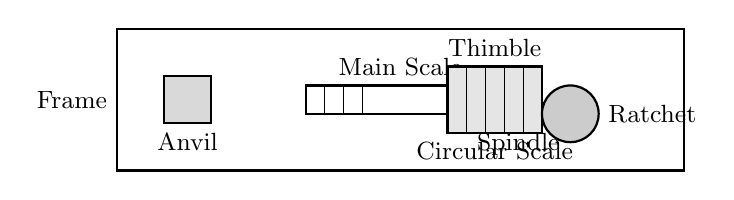
\begin{tikzpicture}[scale=1.2]
    % Frame
    \draw[thick] (0,0) -- (0,1.5) -- (6,1.5) -- (6,0) -- cycle;
    % Anvil
    \fill[gray!30] (0.5,0.5) rectangle (1,1);
    \draw[thick] (0.5,0.5) rectangle (1,1);
    \node[below] at (0.75,0.5) {\small Anvil};
    % Spindle
    \fill[gray!30] (4,0.5) rectangle (4.5,1);
    \draw[thick] (4,0.5) rectangle (4.5,1);
    \node[below] at (4.25,0.5) {\small Spindle};
    % Sleeve (Main Scale)
    \draw[thick] (2,0.6) rectangle (4,0.9);
    \draw (2.2,0.6) -- (2.2,0.9);
    \draw (2.4,0.6) -- (2.4,0.9);
    \draw (2.6,0.6) -- (2.6,0.9);
    \node[above] at (3,0.9) {\small Main Scale};
    % Thimble (Circular Scale)
    \draw[thick,fill=gray!20] (3.5,0.4) rectangle (4.5,1.1);
    \draw (3.7,0.4) -- (3.7,1.1);
    \draw (3.9,0.4) -- (3.9,1.1);
    \draw (4.1,0.4) -- (4.1,1.1);
    \draw (4.3,0.4) -- (4.3,1.1);
    \node[above] at (4,1.1) {\small Thimble};
    \node[below] at (4,0.4) {\small Circular Scale};
    % Ratchet
    \draw[thick,fill=gray!40] (4.8,0.6) circle (0.3);
    \node[right] at (5.1,0.6) {\small Ratchet};
    % Frame label
    \node[left] at (0,0.75) {\small Frame};
\end{tikzpicture}
\caption{Micrometer Screw Gauge}
\end{figure}

\paragraph{Key Parts:}
\begin{enumerate}
    \item \textbf{Frame:} C-shaped rigid body that holds all parts
    \item \textbf{Anvil:} Fixed end against which object is placed
    \item \textbf{Spindle:} Moving part that advances towards anvil
    \item \textbf{Sleeve (Main Scale):} Shows millimeter divisions
    \item \textbf{Thimble (Circular Scale):} Shows fractional divisions (0-50 or 0-100)
    \item \textbf{Ratchet:} Ensures uniform pressure during measurement
\end{enumerate}

\paragraph{Mnemonic:} \emph{Frame-Anvil-Spindle-Sleeve-Thimble-Ratchet (FASSTR).}

\subsection{Question 2(b)(2) [4 marks]}
\textbf{Explain the zero, positive and negative errors for vernier calipers with proper diagram and list necessary steps to remove these types of errors.}

\subsubsection{Solution}
\paragraph{Types of Errors:}

\begin{enumerate}
    \item \textbf{Zero Error:} When the jaws are closed, if the zero of vernier scale does not coincide with zero of main scale, the instrument has zero error.
    
    \item \textbf{Positive Zero Error:} When the zero of vernier scale is to the \textit{right} of the main scale zero. The reading is \textit{more} than actual, so we \textit{subtract} the error.
    
    \item \textbf{Negative Zero Error:} When the zero of vernier scale is to the \textit{left} of the main scale zero. The reading is \textit{less} than actual, so we \textit{add} the error.
\end{enumerate}

\paragraph{Steps to Remove Errors:}
\begin{enumerate}
    \item Note the zero error when jaws are closed
    \item For positive error: Subtract error from measured reading
    \item For negative error: Add the error value to measured reading
    \item Formula: Corrected Reading = Measured Reading - Zero Error
    \item If zero error persists, the instrument needs calibration by a technician
\end{enumerate}

\paragraph{Mnemonic:} \emph{Positive error = Subtract, Negative error = Add.}

\subsection{Question 2(b)(3) [4 marks]}
\textbf{In an experiment of finding the periodic time of a simple pendulum, the observations are 1.96 s, 1.98 s, 2.00 s, 2.02 s, 2.04 s. Calculate absolute error, mean absolute error, relative error and percentage error.}

\subsubsection{Solution}
\paragraph{Given Data:}
Observations: \(T_1 = 1.96\,s\), \(T_2 = 1.98\,s\), \(T_3 = 2.00\,s\), \(T_4 = 2.02\,s\), \(T_5 = 2.04\,s\)

\paragraph{Calculations:}

\subparagraph{Mean Value:}
The mean value is the arithmetic average of all observations:
\[ T_{mean} = \frac{T_1 + T_2 + T_3 + T_4 + T_5}{5} = \frac{1.96 + 1.98 + 2.00 + 2.02 + 2.04}{5} = \frac{10.00}{5} = 2.00\,s \]
This represents the most probable value of the periodic time.

\subparagraph{Absolute Errors:}
Absolute error for each observation is the absolute difference from the mean:
\[ \Delta T_1 = |T_{mean} - T_1| = |2.00 - 1.96| = 0.04\,s \]
\[ \Delta T_2 = |2.00 - 1.98| = 0.02\,s \]
\[ \Delta T_3 = |2.00 - 2.00| = 0.00\,s \]
\[ \Delta T_4 = |2.00 - 2.02| = 0.02\,s \]
\[ \Delta T_5 = |2.00 - 2.04| = 0.04\,s \]

\subparagraph{Mean Absolute Error:}
The mean absolute error is the average of all individual absolute errors:
\[ \Delta T_{mean} = \frac{\Delta T_1 + \Delta T_2 + \Delta T_3 + \Delta T_4 + \Delta T_5}{5} = \frac{0.04 + 0.02 + 0.00 + 0.02 + 0.04}{5} = \frac{0.12}{5} = 0.024\,s \]
This represents the uncertainty in our measurement.

\subparagraph{Relative Error:}
Relative error is the ratio of mean absolute error to mean value:
\[ \text{Relative Error} = \frac{\Delta T_{mean}}{T_{mean}} = \frac{0.024}{2.00} = 0.012 \]
This is a dimensionless quantity that indicates the fractional uncertainty.

\subparagraph{Percentage Error:}
Percentage error expresses relative error as a percentage:
\[ \text{Percentage Error} = \text{Relative Error} \times 100\% = 0.012 \times 100\% = 1.2\% \]

\paragraph{Answers:}
\begin{itemize}
    \item Mean Absolute Error = 0.024 s
    \item Relative Error = 0.012
    \item Percentage Error = 1.2\%
\end{itemize}

\paragraph{Significance:}
A percentage error of 1.2\% indicates high precision in our measurements. The experiment was conducted carefully with minimal random errors.

\paragraph{Mnemonic:} \emph{Mean → Absolute → Relative → Percentage.}

\end{document}
